\documentclass[12pt,a4paper,UTF8]{ctexart}
\usepackage{graphicx}
\usepackage{amsmath}
\usepackage{amssymb}
\usepackage{cite}
\usepackage[ntheorem]{empheq}
\usepackage{enumitem}
\usepackage{fullpage}
\usepackage{tocbibind}
\usepackage[bookmarksopen=true,colorlinks,linkcolor=black]{hyperref}
\usepackage{cellspace}
\usepackage{listings}
\usepackage{color}
\usepackage{epstopdf}
\usepackage{subfigure}
\usepackage{algorithm}
\usepackage{algorithmicx}
\usepackage{algpseudocode}

\renewcommand{\algorithmicrequire}{\textbf{Input:}}  % Use Input in the format of Algorithm
\renewcommand{\algorithmicensure}{\textbf{Output:}} % Use Output in the format of Algorithm
\usepackage{longtable}

\usepackage{float}
\definecolor{gray}{rgb}{0.5,0.5,0.5}
\definecolor{dkgreen}{rgb}{.068,.578,.068}
\definecolor{dkpurple}{rgb}{.320,.064,.680}

% set Matlab styles
\lstset{
   language=Matlab,
   numbers=left,
   keywords={break,case,catch,continue,else,elseif,end,for,function,
      global,if,otherwise,persistent,return,switch,try,while},
   basicstyle=\ttfamily,
   keywordstyle=\color{blue}\bfseries,
   commentstyle=\color{dkgreen},
   stringstyle=\color{dkpurple},
   backgroundcolor=\color{white},
   tabsize=4,
   showspaces=false,
   showstringspaces=false,
}

\begin{document}
\CJKfamily{zhkai}


\begin{center}
    \textbf{作业一}\\
    \textbf{姓名 胡毅翔 ~~ 学号 PB18000290 ~~ 日期 2021年5月4日}\\
\end{center}

\begin{center}
    \fbox{
        \begin{minipage}{40em}
            \vspace{5cm}
            \hspace{20cm}
        \end{minipage}}
\end{center}
\vspace{1cm}

\begin{enumerate}
    \item[第一题] \textbf{求解线性方程的迭代方法}

          本题考虑使用有限差分方法(finite difference method)解决两点边值问题(boundary
          value problem)
          \begin{equation}
              -u^{\prime \prime}(x)=f(x) \quad(0<x<1) \text { 使得 } u(0)=T_{0} \quad \text { and } \quad u(1)=T_{1}
          \end{equation}
          时产生的离散化线性系统
          \begin{equation}
              A x=b
          \end{equation}
          的求解问题。适当选取离散化的步长后我们会得到一个10 × 10的系统:
          \begin{equation}
              A=\left[\begin{array}{rrrrrrrr}
                      2  & -1 &        &        &    &    \\
                      -1 & 2  & -1     &        &    &    \\
                         & -1 & 2      & \ddots &    &    \\
                         &    & \ddots & \ddots & -1 &    \\
                         &    &        & -1     & 2  & -1 \\
                         &    &        &        & -1 & 2
                  \end{array}\right], \quad b=\left[\begin{array}{llllllllll}
                      2 & -2 & 2 & -1 & 0 & 0 & 1 & -2 & 2 & -2
                  \end{array}\right]^{T}
          \end{equation}
          此处,A中空白部分的元素皆为0。我们容易验证上述线性系统的精确解为
          \begin{equation}\label{eq4}
              x_{\text {exact }}=\left[\begin{array}{llllllllll}
                      1 & 0 & 1 & 0 & 0 & 0 & 0 & -1 & 0 & -1
                  \end{array}\right]^{T}
          \end{equation}
          (a) (20分)分别使用Jacobi和Gauss-Siedel方法求解上述问题。利用精确解\eqref{eq4}将误差大小和迭代次数的关系用semilogy图表示出来 (横轴为迭代次数 $n$, 纵轴为迭代解与精确解的差距)。

          Jacobi和Gauss-Siedel方法运行结果见图\ref{4},算法见(b)题代码部分。

          \begin{figure}[H]
              \centering
              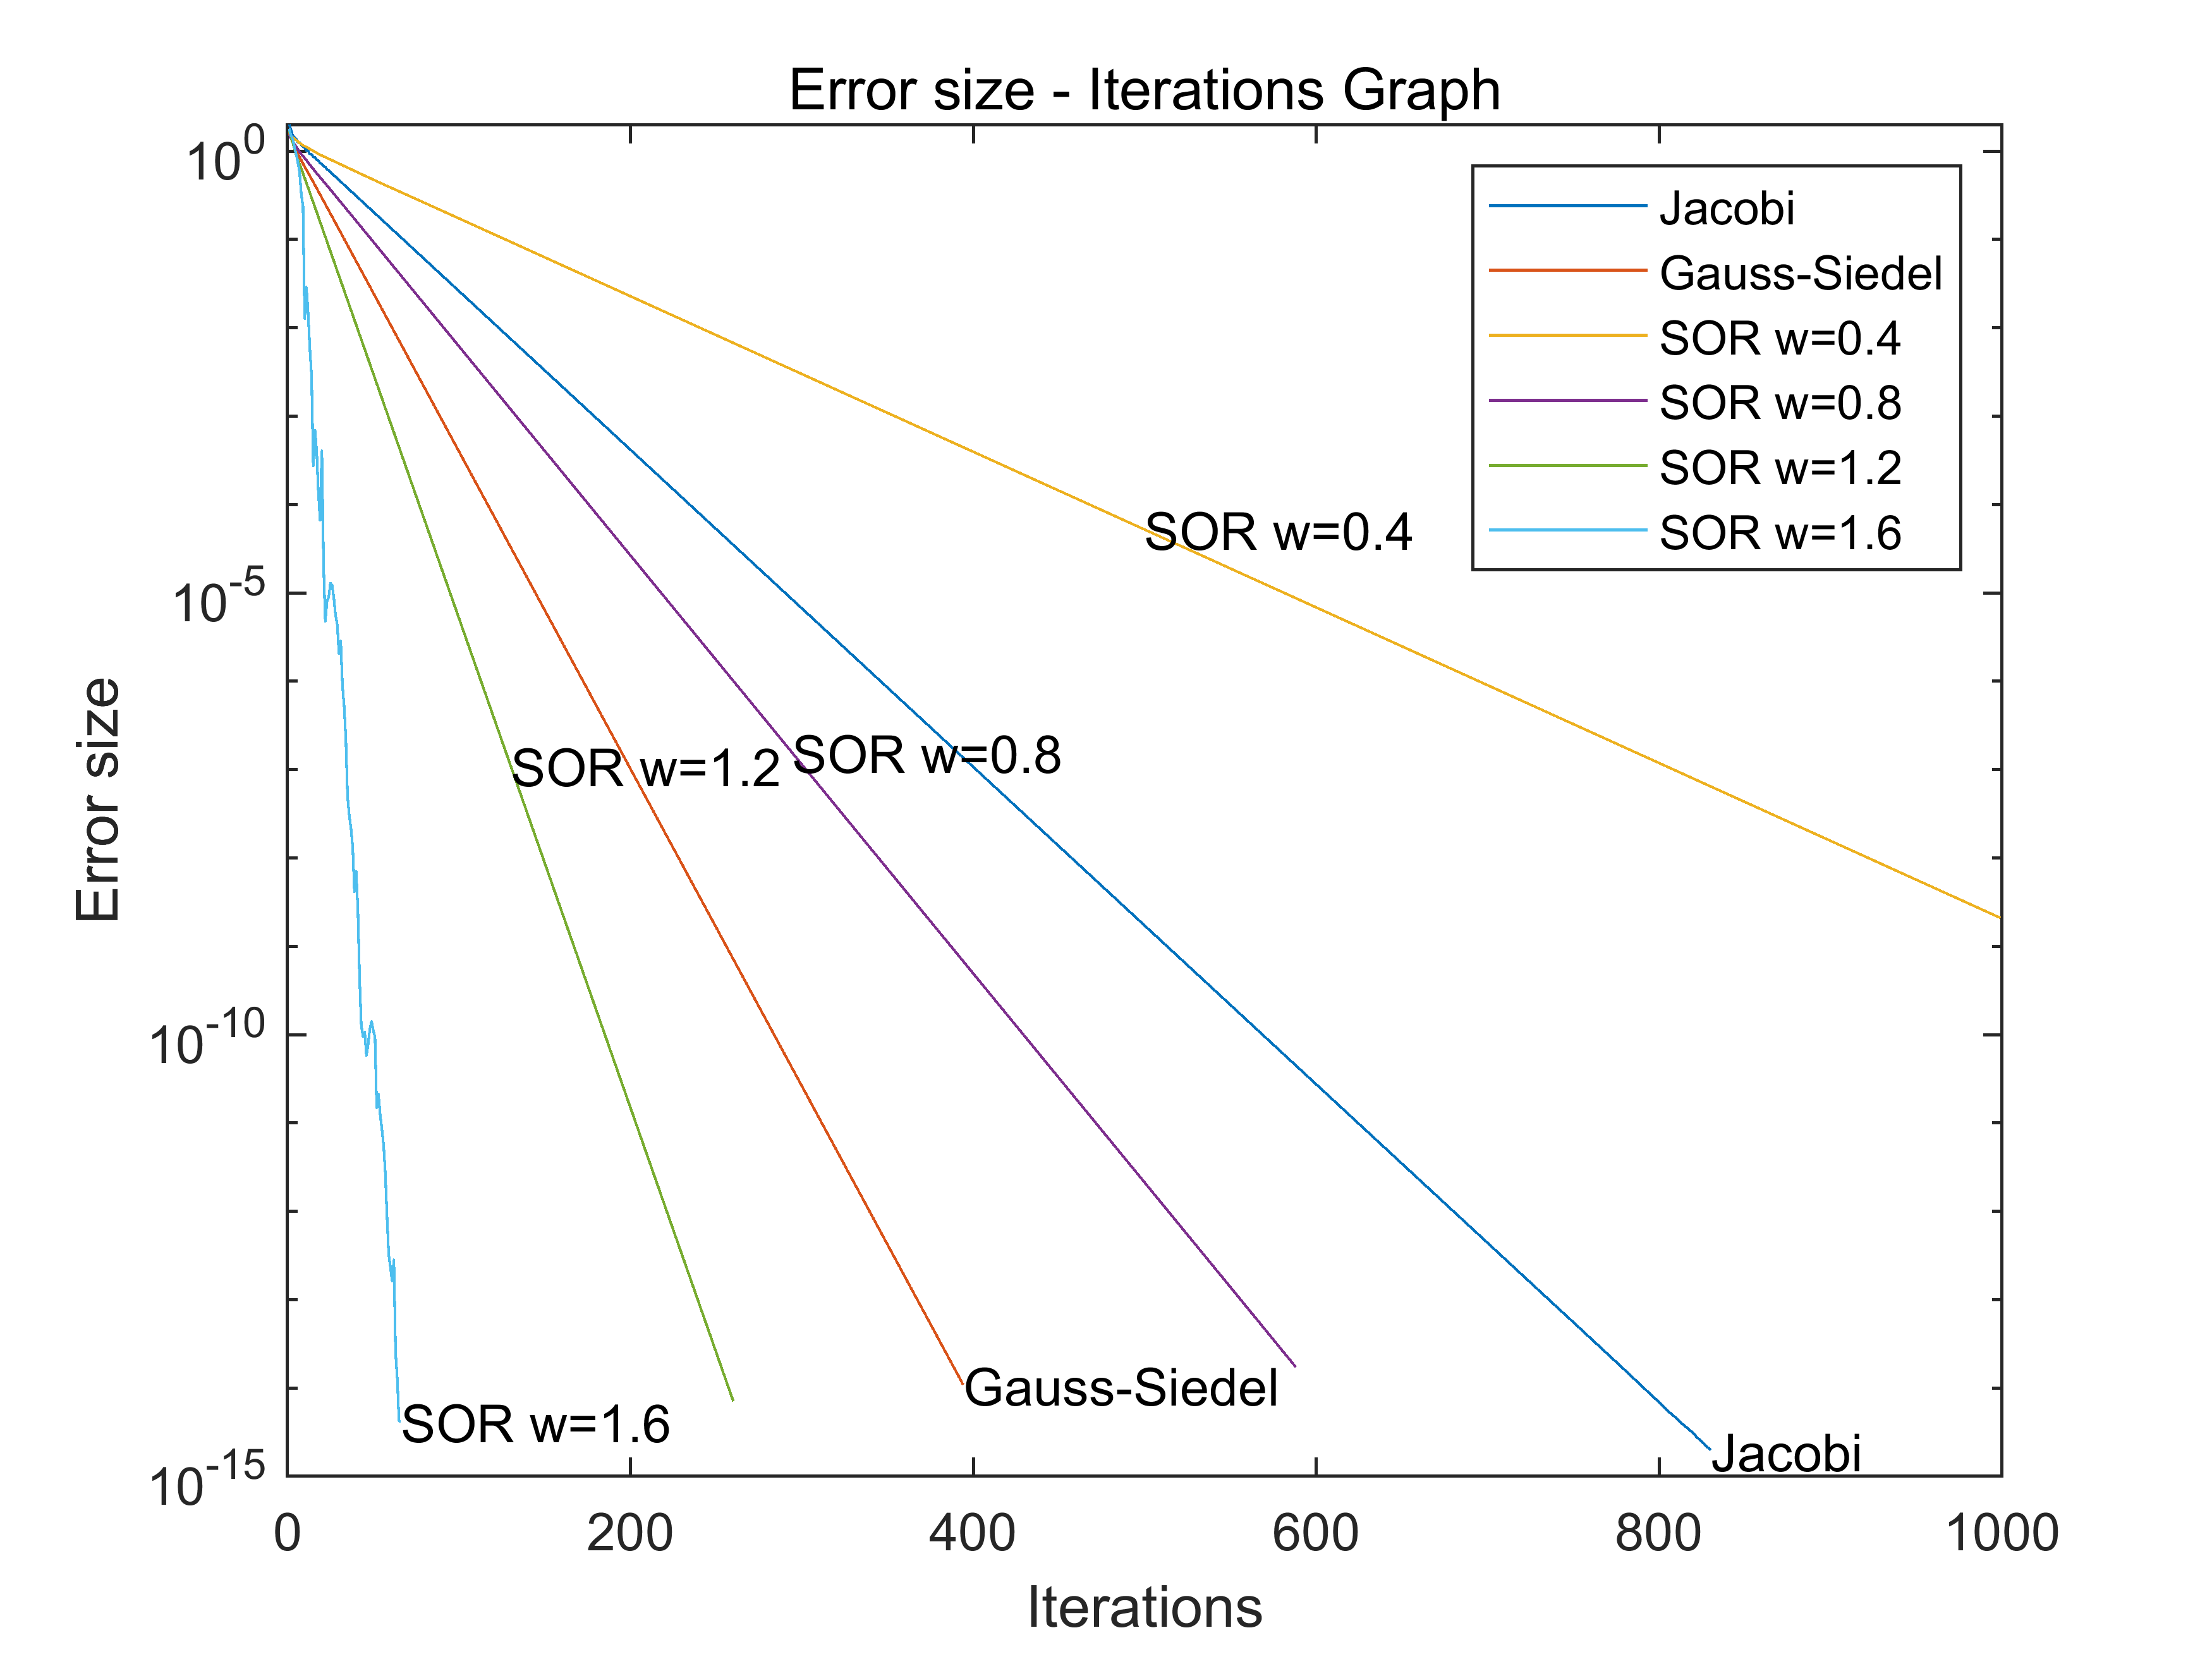
\includegraphics[width=0.8\textwidth]{q.png}
              \caption{迭代方法的误差大小与迭代次数的semilogy图}\label{4}
          \end{figure}
          \begin{figure}[H]
              \centering
              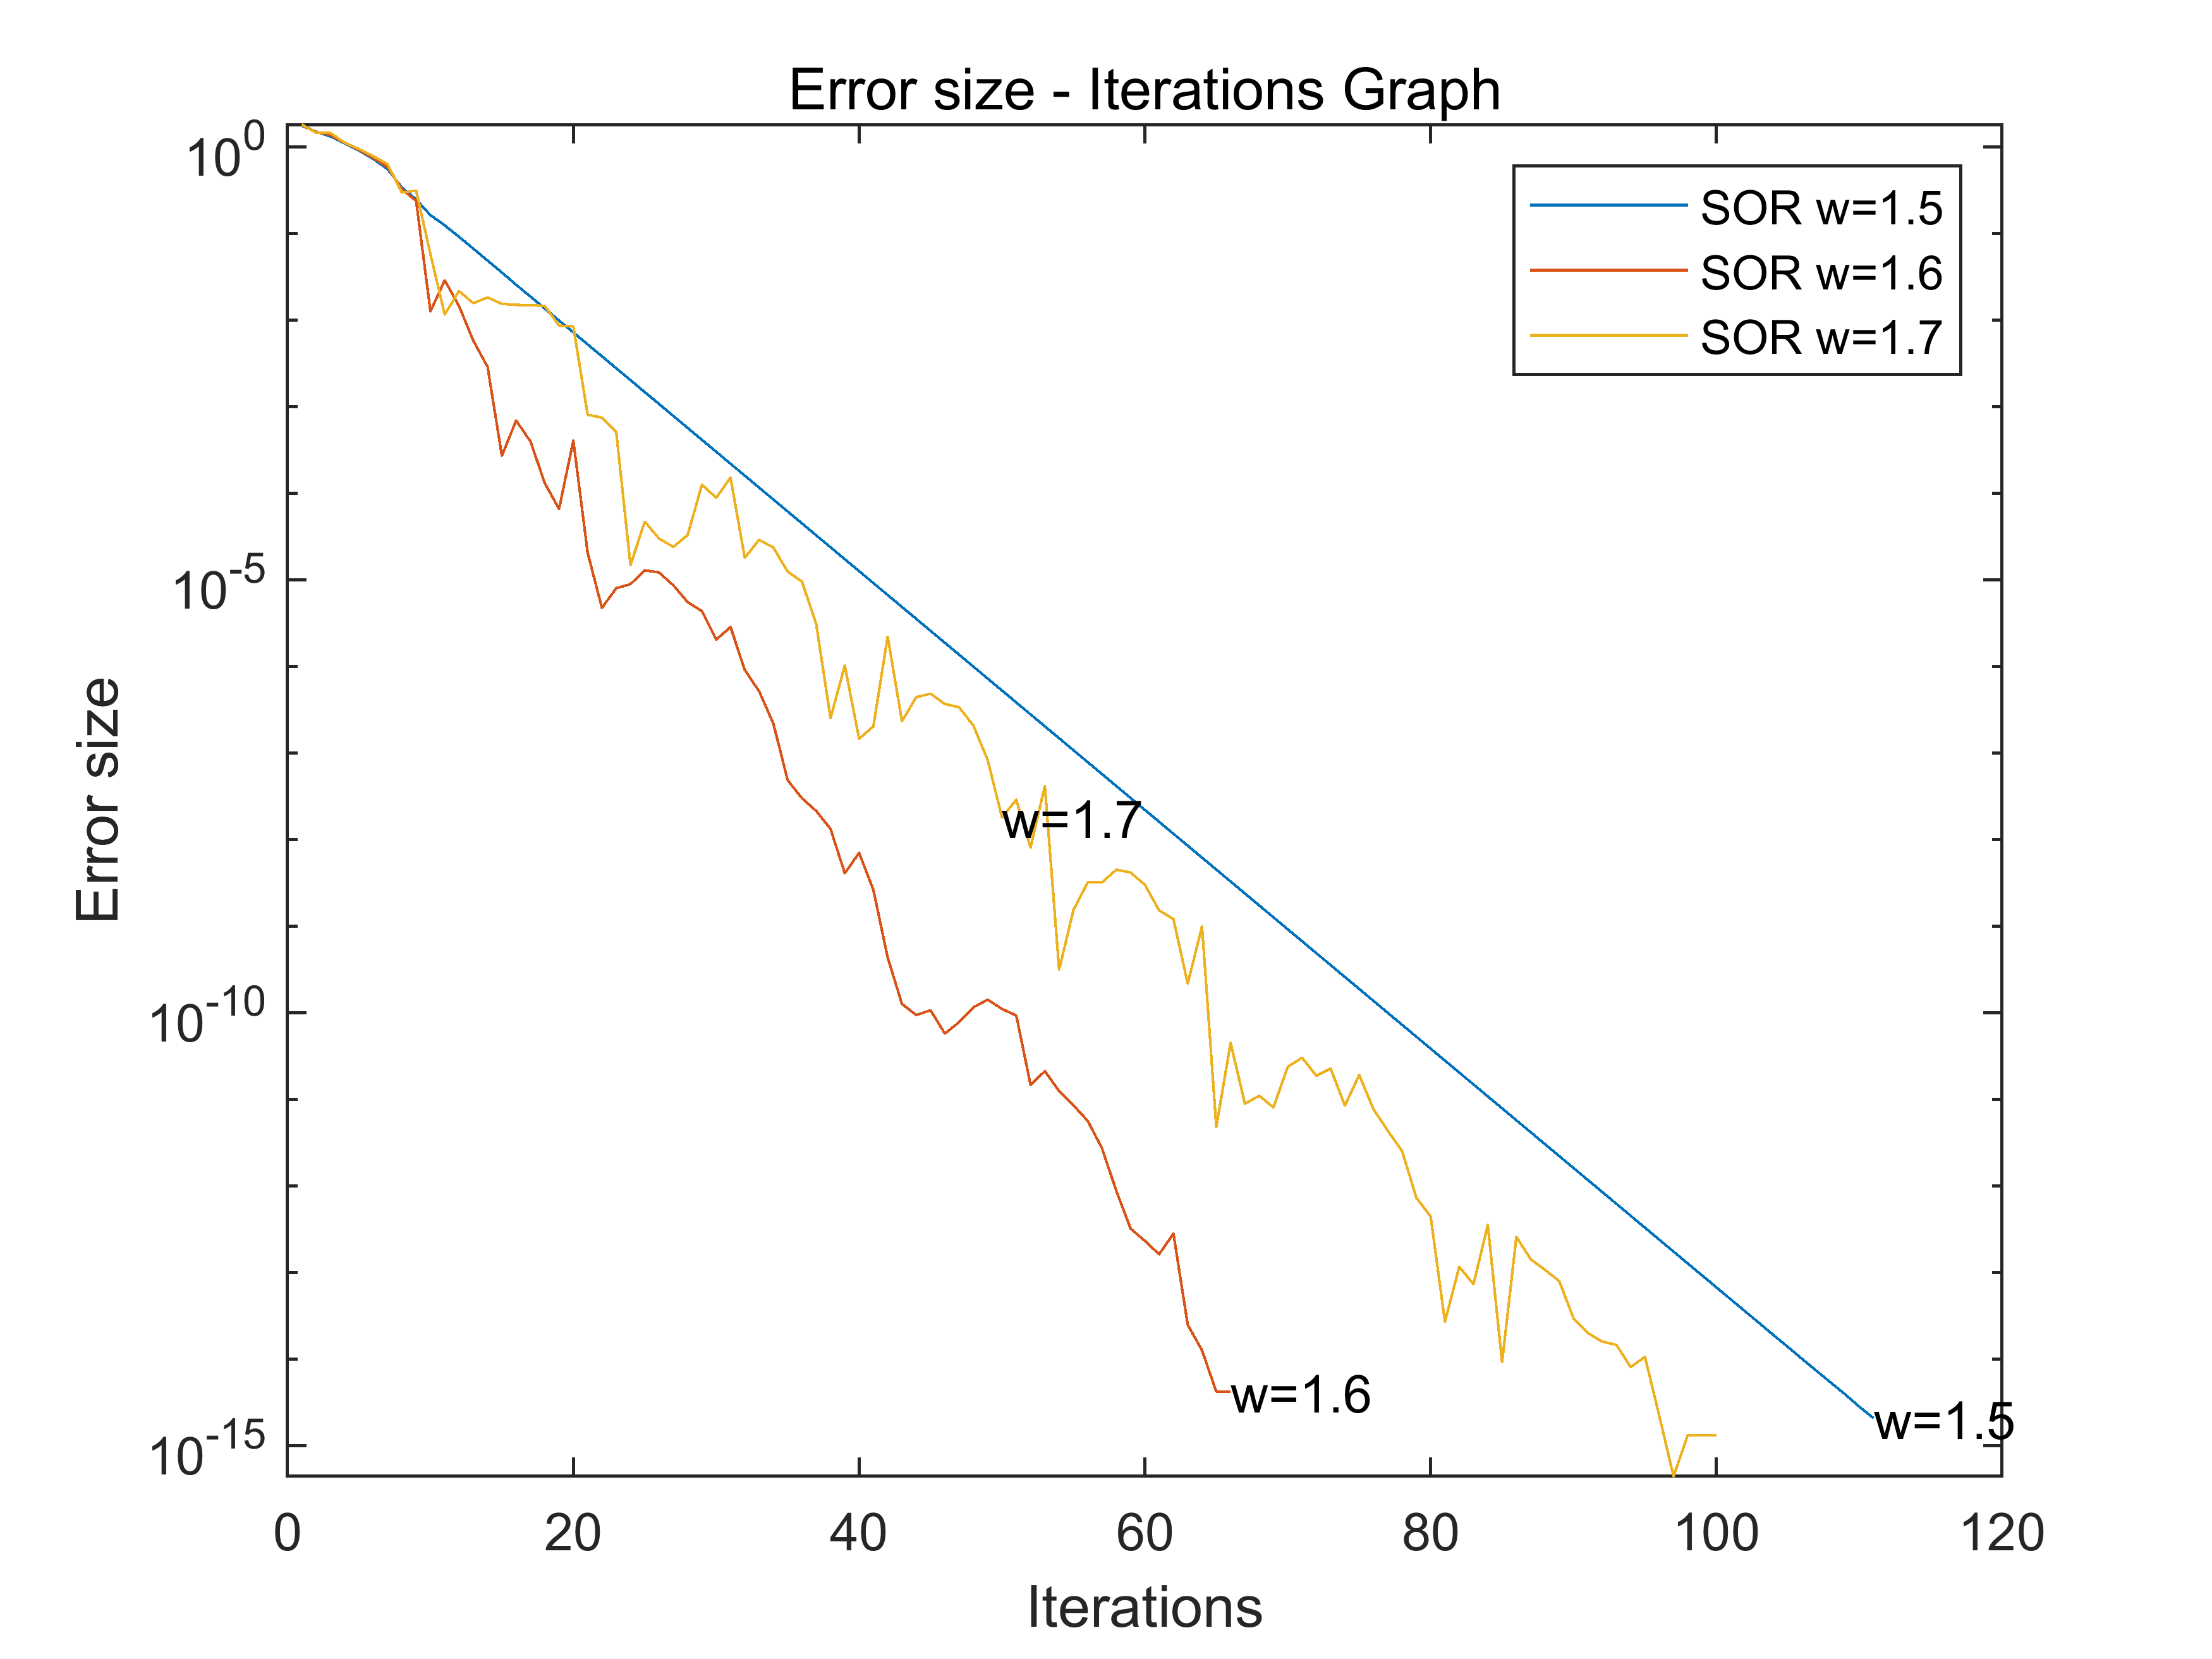
\includegraphics[width=0.8\textwidth]{2.png}
              \caption{不同 $\omega$ 的SOR迭代的误差大小与迭代次数的semilogy图}\label{sor}
          \end{figure}
          (b) (10分)选取若干不同的松他因子 $\omega$ 使用SOR方法解上述问题,并将收敛结果画在上一问的图中。请在图上相应的收敛线旁标示出这些 $\omega$ 的值。以迭代次数做为判断标准,指出对应于10 $^{-15}$ 的误差目标哪个大概的 $\omega$ 值收敛速度最快。

          由图\ref{4}分析,在 $\omega = 1.6$ 时收敛速度较快。在图\ref{sor}中,将 $\omega = 1.5, 1.6, 1.7$ 进行比较,得出结论:

          在本题所给的数据下,对应于10$^{-15}$ 的误差目标,$\omega = 1.6$ 时收敛速度较快。

          注:本题代码部分为绘制图\ref{4}所用的代码,绘制图\ref{sor}只需调用其中的SOR函数,修改参数 $\omega$ 的值并重新绘图即可。根据报告从简原则,不再重复。

          (a),(b)两题所用\textsc{Matlab}程序显示如下:
          \begin{lstlisting}[frame=single]
clear, clc;
% The value of A and B:
A = [2, -1, 0, 0, 0, 0, 0, 0, 0, 0;
    -1, 2, -1, 0, 0, 0, 0, 0, 0, 0;
    0, -1, 2, -1, 0, 0, 0, 0, 0, 0;
    0, 0, -1, 2, -1, 0, 0, 0, 0, 0;
    0, 0, 0, -1, 2, -1, 0, 0, 0, 0;
    0, 0, 0, 0, -1, 2, -1, 0, 0, 0;
    0, 0, 0, 0, 0, -1, 2, -1, 0, 0;
    0, 0, 0, 0, 0, 0, -1, 2, -1, 0;
    0, 0, 0, 0, 0, 0, 0, -1, 2, -1;
    0, 0, 0, 0, 0, 0, 0, 0, -1, 2];
b = [2; -2; 2; -1; 0; 0; 1; -2; 2; -2];
epsilon = 10^(-15);
% Jacobi Part:
x_exact = [1; 0; 1; 0; 0; 0; 0; -1; 0; 1];
tmp = abs(max(x_exact));
x_1 = [0; 0; 0; 0; 0; 0; 0; 0; 0; 0];
x_2 = [1; 1; 1; 1; 1; 1; 1; 1; 1; 1];
% initialization
D = diag(diag(A));
R = speye(10) - D \ A;
g = D \ b;
count_J = []; % count: used to save the error size
number_J = 1; % Iterations

while abs(max(x_1 - x_2)) > epsilon
    x_1 = x_2;
    x_2 = R * x_1 + g;
    count_J(number_J) = abs(max(x_2 - x_exact)) / tmp;
    number_J = number_J + 1;
end

% Print the output of Jacobi
x = x_2

% Gauss-Siedel Part:
x_1 = [0; 0; 0; 0; 0; 0; 0; 0; 0; 0];
x_2 = [1; 1; 1; 1; 1; 1; 1; 1; 1; 1];
% initialization
L = tril(A, -1);
U = triu(A, 1);
D = diag(diag(A));
S = -(D + L) \ U;
f = (D + L) \ b;
count_G = []; % count: used to save the error size
number_G = 1; % Iterations

while abs(max(x_1 - x_2)) > epsilon
    x_1 = x_2;
    x_2 = S * x_1 + f;
    count_G(number_G) = abs(max(x_2 - x_exact)) / tmp;
    number_G = number_G + 1;
end

% Print the output of Gauss-Siedel
x = x_2

% SOR Part:
% w=0.4:
[count_S_0, x, state] = SOR(0.4, A, x_exact, b);
% w=0.8:
[count_S_1, x, state] = SOR(0.8, A, x_exact, b);
% w=1.2:
[count_S_2, x, state] = SOR(1.2, A, x_exact, b);
% w=1.6:
[count_S_3, x, state] = SOR(1.6, A, x_exact, b);
semilogy([1:length(count_J)], count_J, ...
    [1:length(count_G)], count_G, ...
    [1:length(count_S_0)], count_S_0, ...
    [1:length(count_S_1)], count_S_1, ...
    [1:length(count_S_2)], count_S_2, ...
    [1:length(count_S_3)], count_S_3);
legend('Jacobi', 'Gauss-Siedel', 'SOR w=0.4', ...
    'SOR w=0.8', 'SOR w=1.2', 'SOR w=1.6', ...
    'Location', 'northeast');
xlabel('Iterations');
ylabel('Error size');
title('Error size - Iterations Graph');
text(length(count_J), ...
    count_J(length(count_J)), 'Jacobi');
text(length(count_G), ...
    count_G(length(count_G)), 'Gauss-Siedel');
text(length(count_S_0) / 2, ...
    count_S_0(floor(length(count_S_0) / 2)), 'SOR w=0.4');
text(length(count_S_1) / 2, ...
    count_S_1(length(count_S_1) / 2), 'SOR w=0.8');
text(length(count_S_2) / 2, ...
    count_S_2(length(count_S_2) / 2), 'SOR w=1.2');
text(length(count_S_3), ...
    count_S_3(length(count_S_3)), 'SOR w=1.6');

function [count, x, state] = SOR(w, A, x, b)
    x_exact = x;
    tmp = abs(max(x_exact));
    x_1 = [0; 0; 0; 0; 0; 0; 0; 0; 0; 0];
    x_2 = [1; 1; 1; 1; 1; 1; 1; 1; 1; 1];
    % initialization
    L = tril(A, -1);
    U = triu(A, 1);
    D = diag(diag(A));
    D_INV = inv(D);
    epsilon = 10^(-15);
    S = (speye(10) + w * D_INV * L) \ ...
(speye(10) - w * (D_INV * U + speye(10)));
    f = w * inv(speye(10) + w * D_INV * L) * (D_INV * b);
    count = []; % count: used to save the error size
    number = 1; % Iterations

    while abs(max(x_1 - x_2)) > epsilon & number < 1000
        x_1 = x_2;
        x_2 = (S * x_1 + f);
        count(number) = abs(max(x_2 - x_exact)) / tmp;
        number = number + 1;
    end
    % if not convergence, return state = 0
    if number == 1000
        state = 0
    else
        state = 1
        % Print the output of SOR 
        x_2
    end

end
         \end{lstlisting}
          (c) (15分)注意到题目中的矩阵A是一个稀疏矩阵(sparse matrix),即有大量元素为0的矩阵。更改你的程序,省略那些和零元素相关的运算
          ,使得你的程序得到加速。使用MATLAB中的tic和toc命令统计上述三种方法得到较为精确的解的时候的计算用时,并和改进后的程序的(在使用
          相同迭代次数的情况下的)耗时列表做对比(左边一列为未加速的程序的计算时间,右边一列为加速后的时间)。注意你需要将每种方法反复运行$N$
          次(比如10次)然后忽略第一次的运行时间,求后面 $N-1$ 次运行时间的平均值或者总和。这是由于MATLAB需要在第一次运算时对程序进行编译并分
          配存储空间。这类花费被统称为overhead, 中文有时会勉强地将其译为“额外开销"。

          因为迭代过程中的主要开销来自循环中对新的$\overrightarrow{X^{k+1}}$的计算,其中迭代矩阵和$\overrightarrow{X^{k}}$的乘法计算开销较大。
          因此,优化的思路为将乘法展开,只对非零元素进行计算。

          对于Jacobi, Gauss-Siedel, SOR方法,迭代矩阵的非零元分布如下:
          \begin{figure}[H] \centering
              \subfigure[Jacobi] {
                  \label{fig:a}
                  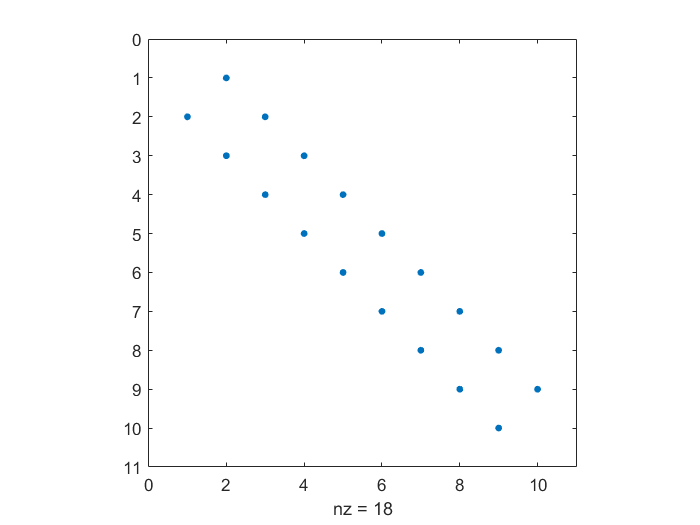
\includegraphics[width=0.2\columnwidth]{j.png}
              }
              \subfigure[Gauss-Siedel] {
                  \label{fig:b}
                  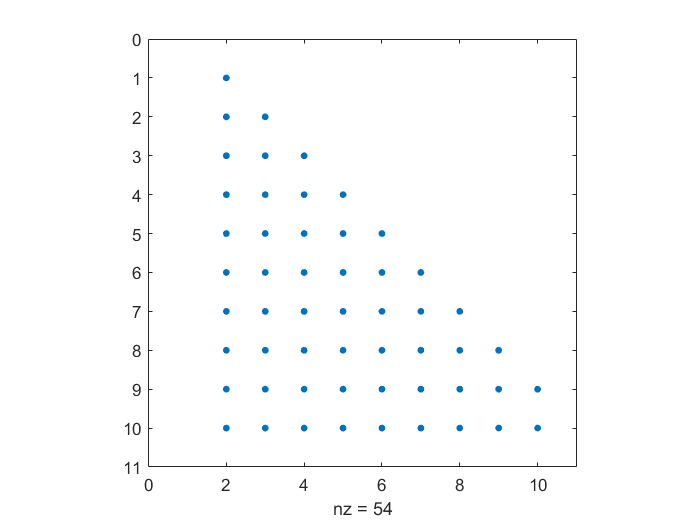
\includegraphics[width=0.2\columnwidth]{G.png}
              }
              \subfigure[SOR] {
                  \label{fig:b}
                  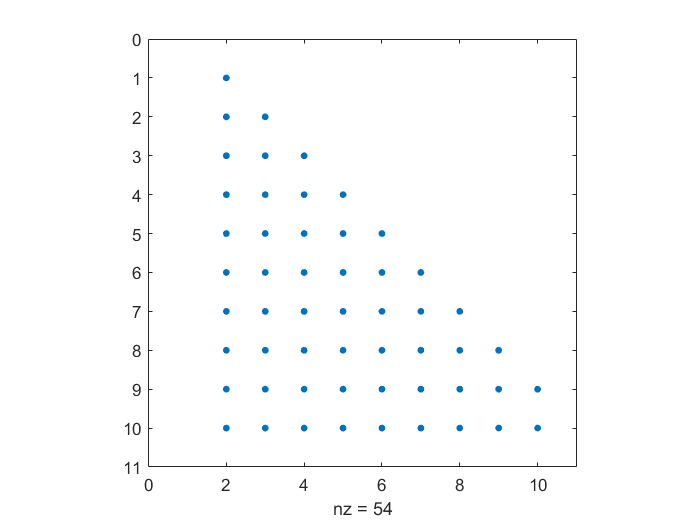
\includegraphics[width=0.2\columnwidth]{G.png}
              }
              \caption{不同方法的迭代矩阵的非零元分布}
              \label{fig}
          \end{figure}


          根据非零元分布,设计优化算法,见代码部分,优化前后花销如表\ref{tb1}。可以看出优化效果并不明显,甚至有的方法优化后时间开销反而更长。这与\textsc{Matlab}的底层实现有关,可能对原来的矩阵乘法有并行化的处理。
          \begin{table}[H]
              \centering
              \begin{tabular}{|c|c|c|}
                  \hline
                  \textbf{Iterative method} & \textbf{Before optimization} & \textbf{After optimization} \\ \hline
                  Jacobi                    & 0.645113                     & 0.588853                    \\ \hline
                  Gauss-Siedel              & 0.361099                     & 0.470360                    \\ \hline
                  SOR $\omega$=1.6          & 0.095594                     & 0.121773                    \\ \hline
              \end{tabular}
              \caption{不同迭代方法优化前后迭代$1000$次所用时间表(单位:s)}
              \label{tb1}
          \end{table}
          (c)题所用\textsc{Matlab}程序显示如下:
          \begin{lstlisting}[frame=single]
% Jacobi Part:

while abs(max(x_1 - x_2)) > 10^(- 15)
    x_1 = x_2;
    x_2(1) = R(1, 2) * x_1(2);

    for i = 2:9
        x_2(i) = R(i, i - 1) * x_1(i - 1) + ...
            R(i, i + 1) * x_1(i + 1);
    end

    x_2(10) = R(10, 9) * x_1(9);
    x_2 = x_2 + g;
    %x_2 = R * x_1 + g;
    count_J(number_J) = abs(max(x_2 - x_exact)) / tmp;
    number_J = number_J + 1;
end

% Gauss-Siedel Part:

while abs(max(x_1 - x_2)) > 10^(- 15)
    x_1 = x_2;

    for i = 1:9
        x_2(i) = 0;

        for j = 2:i + 1
            x_2(i) = x_2(i) + S(i, j) * x_1(j);
        end

    end

    x_2(10) = 0;

    for j = 2:10
        x_2(10) = x_2(10) + S(10, j) * x_1(j);
    end

    x_2 = x_2 + f;
    count_G(number_G) = abs(max(x_2 - x_exact)) / tmp;
    number_G = number_G + 1;
end

% SOR Part:

while abs(max(x_1 - x_2)) > 10^(- 15) & number < 1000
    x_1 = x_2;

    for i = 1:9
        x_2(i) = 0;

        for j = 1:i + 1
            x_2(i) = x_2(i) + S(i, j) * x_1(j);
        end

    end

    x_2(10) = 0;

    for j = 1:10
        x_2(10) = x_2(10) + S(10, j) * x_1(j);
    end

    x_2 = x_2 + f;
    count(number) = abs(max(x_2 - x_exact)) / tmp;
    number = number + 1;
end

\end{lstlisting}


    \item[第二题]\textbf{Newton法求解线性方程}

          本题将利用求解方程
          \begin{equation}\label{zhl}
              x^{3}-3 x^{2}+2=0
          \end{equation}
          的根来深入我们关于Newton方法的收敛速度的讨论。容易验证\eqref{zhl}的三个根分别位于 $[-3,0],[0,2],[2,4]$ 三个区间内。我们依从左向右的顺序分别称这三个根为 $x_{l}, x_{m}, x_{r}$。

          (a) (10分)适当选取迭代的初始点,写程序用Newton法求解这三个根,并将每一步迭代的新的近似值打印出来。

          (b) (10分)设计一个估计收敛阶数的方法,在上一问求解的过程中同时求出大概的收敛阶数。

          收敛阶数的估计,可用每一步计算出来的近似值作为精确解的估计,具体如下:
          \begin{equation}
              \alpha \approx \frac{\log \left|\left(x_{n+1}-x_{n}\right) /\left(x_{n}-x_{n-1}\right)\right|}{\log \left|\left(x_{n}-x_{n-1}\right) /\left(x_{n-1}-x_{n-2}\right)\right|}
          \end{equation}
          对于三个根分别选取起始点,每步近似值及收敛阶数如下。
          \begin{table}[H]
              \centering
              \begin{tabular}{|c|c|c|}
                  \hline
                  \textbf{Iter} & \textbf{x}          & \textbf{order}     \\ \hline
                  1             & -1.8444444444444446 &                    \\ \hline
                  2             & -1.1637243901747001 & 1.3714391501568288 \\ \hline
                  3             & -0.8342806448688520 & 1.7240301893065662 \\ \hline
                  4             & -0.7400073072593034 & 1.9813265535540170 \\ \hline
                  5             & -0.7321050507279875 & 2.0094284562727243 \\ \hline
                  6             & -0.7320508101168153 & 2.0005928692388242 \\ \hline
                  7             & -0.7320508075688773 & 2.0000020944499259 \\ \hline
                  8             & -0.7320508075688773 & 2.0000000000492029 \\ \hline
              \end{tabular}
              \caption{每步近似值及收敛阶数(选取$x_{l}=-3$为起始点)}
          \end{table}

          \begin{table}[H]
              \centering
              \begin{tabular}{|c|c|c|}
                  \hline
                  \textbf{Iter} & \textbf{x}         & \textbf{order}     \\ \hline
                  1             & 0.8888888888888888 &                    \\ \hline
                  2             & 1.0009259259259260 & 2.8269574598756742 \\ \hline
                  3             & 0.9999999994707780 & 2.9973992898742279 \\ \hline
                  4             & 1.0000000000000000 & 2.9999999403585704 \\ \hline
                  5             & 1.0000000000000000 & 3.0000000000000000 \\ \hline
              \end{tabular}
              \caption{每步近似值及收敛阶数(选取$x_{m}=1.5$为起始点)}
          \end{table}

          \begin{table}[H]
              \centering
              \begin{tabular}{|c|c|c|}
                  \hline
                  \textbf{Iter} & \textbf{x}         & \textbf{order}     \\ \hline
                  1             & 2.7777777777777777 &                    \\ \hline
                  2             & 2.7337566137566136 & 2.0087046715549723 \\ \hline
                  3             & 2.7320533217303780 & 2.0043558409397728 \\ \hline
                  4             & 2.7320508075743515 & 2.0000999497969754 \\ \hline
                  5             & 2.7320508075688772 & 2.0000000742240944 \\ \hline
                  6             & 2.7320508075688772 & 2.0000000000000808 \\ \hline
              \end{tabular}
              \caption{每步近似值及收敛阶数(选取$x_{r}=3$为起始点)}
          \end{table}

          (c) (10分)Newton是一个二阶收敛的方法。上一问中你是否观测到了比二阶收敛更快的现象?如果有,请尽可能详细地解释其原因。

          其中,在求$x_{m}$时,出现了比二阶收敛更快的现象,收敛阶数约为3。可能的原因为:
          \begin{equation}
              f(x)=x^{3}-3 x^{2}+2
          \end{equation}
          求二阶导:
          \begin{equation}\label{zhll}
              f^{\prime \prime}(x)=6 x-6
          \end{equation}
          又由:
          \begin{equation}\label{EQ8}
              0=f(\xi )=f(x_{n})+(\xi -x_{n})f^{\prime}(x_{n})+\frac{(\xi -x_{n})_{2}}{2}f^{\prime \prime}(\eta_{n})
          \end{equation}
          可得:
          \begin{equation}
              \frac{\xi - x_{n+1}}{(\xi - x_{n})^{2}} = -\frac {f^{\prime \prime}(\eta_{n})}{2f^{\prime}(x^{n})}
          \end{equation}
          由\eqref{zhll}知,$f^{\prime \prime}(1)=0$。故\eqref{EQ8},退化为:
          \begin{equation}\label{EQ10}
              0=f(\xi )=f(x_{n})+(\xi -x_{n})f^{\prime}(x_{n})+\frac{(\xi -x_{n})^{2}}{2}f^{\prime \prime}(x_{n})+\frac{(\xi -x_{n})^{3}}{6}f^{\prime \prime \prime}(\eta_{n})
          \end{equation}
          可得:
          \begin{equation}
              \frac{\xi - x_{n+1}}{(\xi - x_{n})^{3}} \approx -\frac {f^{\prime \prime \prime}(\eta_{n})}{6f^{\prime}(x_{n})}
          \end{equation}
          即收敛阶数约为3,与数据实验结果相符。

          (a)(b)两题所用\textsc{Matlab}程序显示如下:
          \begin{lstlisting}[frame=single]
clear,clc;
syms x;
maxrept = 1000;
f(x) = x^3 - 3 * x^2 + 2; %Equation to be solved
g(x) = diff(f, x); %df/dx
epsilon = 10^(-15);

fprintf("set x_l=-3,find out x_l in [-3,0]\n");
x_l = Newton(-3, f, g, epsilon, maxrept);
fprintf("The answer of x_l is %.16f\n", x_l);
fprintf("set x_m=1.5,find out the answer in [0,2]\n");
x_m = Newton(1.5, f, g, epsilon, maxrept);
fprintf("The answer of x_m is %.16f\n", x_m);
fprintf("set x_r=3,find out the answer in [2,4]\n");
x_r = Newton(3, f, g, epsilon, maxrept);
fprintf("The answer of x_m is %.16f\n", x_r);

function x = Newton(x_0, f, g, epsilon, maxrept)
    x_1 = x_0 - (f(x_0) / g(x_0));
    fprintf("iter        x                    order\n");

    for i = 1:maxrept
        x_2 = x_1 - (f(x_1) / g(x_1));

        if i >= 2
            % Calculate the order of convergence
            order_0 = order_1;
            order_1 = log(abs(x_2 - x_1) / ...
                abs(x_1 - x_0));
            Alpha = order_1 / order_0;
            fprintf("%d        %.16f     %.16f\n", ...
                i, x_1, Alpha);
        else
            % First iteration
            order_1 = log(abs(x_2 - x_1) / ...
                abs(x_1 - x_0));
            fprintf("%d        %.16f     \n", i, x_1);
        end

        % convergence or not
        if abs(x_1 - x_0) < epsilon
            break
        end

        % update
        x_0 = x_1;
        x_1 = x_2;
    end

    x = x_1;

end


\end{lstlisting}

    \item[第三题]\textbf{幂法求解特征值问题}

          (a) (15分)设计一个能够求解问题存在一个(绝对值意义下的)最大特征值和存在最大的两个特征值,大小相同但符号相反的情况的算法并仿照课堂上所介绍的伪代码的格式写出一个清晰易懂的伪代码。

          \begin{algorithm}[H]
              \caption{Power Iteration to Find Matrix Eigenvalues}
              \label{alg::conjugateGradient}
              \begin{algorithmic}[1]
                  \Require
                  $A$: Matrix;

                  $maxrept$: the maximum number of iterations;

                  $\varepsilon $: error size;

                  $\overrightarrow{q^{old}} $: initial solution;
                  \Ensure
                  $\lambda$: the eigenvalue of $A$ which has the largest magnitude;

                  $\overrightarrow{\overline{q^{new}} }$: the eigenvector of $\lambda$;

                  $error message$: if the input cannot be resolved by algorithm;
                  \State $\overrightarrow{\overline{q^{old}}}$ $\leftarrow$ ${\overrightarrow{q^{old}}}$/${\left\lVert \overrightarrow{q^{old}}\right\rVert_{\infty} }$;
                  \For {$i$ = $1$ \textbf{to} $maxrept$ }
                  \State$\overrightarrow{q^{update}} $ $\leftarrow$ $A$ $\overrightarrow{\overline{q^{old}}}$;
                  \State$find$ $j$ $that$ $satisfy$ $\left\lvert\overrightarrow{q^{update}}_{j} \right\rvert $=${\left\lVert \overrightarrow{q^{update}}\right\rVert_{\infty} }$;
                  \State$index$ $\leftarrow$ $j$ ;
                  \State$flag$ $\leftarrow$ $\overrightarrow{q^{update}}_{index}$;
                  \State$\overrightarrow{q^{new}}$ $\leftarrow$ $A$ $\overrightarrow{q^{update}}$;
                  \State$\lambda^{2}$ $\leftarrow$ ${\left\lVert \overrightarrow{q^{new}}\right\rVert_{\infty} }$;
                  \State$\overrightarrow{\overline{q^{new}} }$ $\leftarrow$ $\overrightarrow{q^{new}}$ / $\lambda^{2}$;
                  \If{${\left\lVert \overrightarrow{\overline{q^{new}} }-\overrightarrow{\overline{q^{old}} }\right\rVert_{\infty} }$ \textless ~$ \varepsilon $ \textbf{and} $flag$ \textgreater ~$ 0$ }
                  \State\Return{$\sqrt{\lambda^{2}}$, $\overrightarrow{\overline{q^{new}} }$, \textbf{exit}}
                  \ElsIf{${\left\lVert \overrightarrow{\overline{q^{new}} }-\overrightarrow{\overline{q^{old}} }\right\rVert_{\infty} }$ \textless ~$ \varepsilon $ \textbf{and} $flag$ \textless ~$ 0$ }
                  \State\Return{$-\sqrt{\lambda^{2}}$, $\overrightarrow{\overline{q^{new}} }$, \textbf{exit}}
                  \Else
                  \State$\overrightarrow{\overline{q^{old}}}$ $\leftarrow$ $\overrightarrow{\overline{q^{new}}}$ ;
                  \EndIf
                  \EndFor
                  \State \textbf{error message};
              \end{algorithmic}
          \end{algorithm}
          (b)(c)两题所用\textsc{Matlab}程序显示如下:
          \begin{lstlisting}[frame=single]
clc, clear;
% Input of 3(c)
B = [222, 580, 584, 786;
    -82, -211, -208, -288;
    37, 98, 101, 132;
    -30, -82, -88, -109];
% Input of 3(b)
A = [-148, -105, -83, -67;
    488, 343, 269, 216;
    -382, -268, -210, -170;
    50, 38, 32, 29];
A = -A; %comment this line to slove 3(b)
% or uncomment to solve 3(c)
% or add minus to solve -A
q_old = [1; 1; 1; 1];
maxrept = 10000;
epsilon = 10^(-15);
q_old_bar = q_old / max(abs(q_old));
% Calculate eigenvalues by Matlab
eig(A)
% Iterations
for i = 1:maxrept
    q_update = A * q_old_bar;
    [~, I] = max(abs(q_update));
    lamda = q_update(I);
    q_new = A * q_update;
    lamda_square = max(abs(q_new));
    q_new_bar = q_new / lamda_square;

    if max(abs(q_old_bar - q_new_bar)) < epsilon & ...
            lamda > 0
        % Print lambda and eigenvector
        fprintf("lamda:%.16f\nq_new_bar:", ...
            sqrt(lamda_square));
        q_new_bar
        break
    elseif max(abs(q_old_bar - q_new_bar)) < epsilon & ...
            lamda < 0
        % Print lambda and eigenvector
        fprintf("lamda:%.16f\nq_new_bar:", ...
            -sqrt(lamda_square));
        q_new_bar
        break
    else
        q_old_bar = q_new_bar;
    end

end

% error case
if i == maxrept + 1
    fprintf("error message");
end

        \end{lstlisting}
          (b) (10分)用程序实现上一问中你设计的算法,用于求解
          \begin{equation}
              A=\left[\begin{array}{rrrr}
                      -148 & -105 & -83  & -67  \\
                      488  & 343  & 269  & 216  \\
                      -382 & -268 & -210 & -170 \\
                      50   & 38   & 32   & 29
                  \end{array}\right]
          \end{equation}


          的模最大的特征值和特征向量(你提供的特征向量的 $\infty$ -范数应为1)。如果用你的程序求一 $A$ 的模最大的特征值和特征向量呢?你需要保证你的程序对负值的特征值也有效。

          $A$ 的模最大的特征值和特征向量:
          \begin{equation}
              \lambda = 7.9999999999994875
          \end{equation}
          \begin{equation}
              \overrightarrow{\overline{q^{new}} }=\left(\begin{array}{c}
                      -0.310344827586208 \\
                      1.000000000000000  \\
                      -0.793103448275865 \\
                      0.137931034482763
                  \end{array}\right)
          \end{equation}
          $-A$ 的模最大的特征值和特征向量:
          \begin{equation}
              \lambda = -7.9999999999994875
          \end{equation}
          \begin{equation}
              \overrightarrow{\overline{q^{new}} }=\left(\begin{array}{c}
                      -0.310344827586208 \\
                      1.000000000000000  \\
                      -0.793103448275865 \\
                      0.137931034482763
                  \end{array}\right)
          \end{equation}
          (c) (10分)用程序实现第一问中你设计的算法,用于求解
          \begin{equation}
              \left[\begin{array}{rrrr}
                      222 & 580  & 584  & 786  \\
                      -82 & -211 & -208 & -288 \\
                      37  & 98   & 101  & 132  \\
                      -30 & -82  & -88  & -109
                  \end{array}\right]
          \end{equation}
          的模最大的特征值和特征向量(你提供的特征向量的$\infty$ -范数应为1)。

          $A$ 的模最大的特征值和特征向量:
          \begin{equation}
              \lambda = 4.9999999999996785
          \end{equation}
          \begin{equation}
              \overrightarrow{\overline{q^{new}} }=\left(\begin{array}{c}
                      -1.000000000000000 \\
                      0.285714285714289  \\
                      -0.178571428571430 \\
                      0.214285714285712
                  \end{array}\right)
          \end{equation}
          $-A$ 的模最大的特征值和特征向量:
          \begin{equation}
              \lambda = -4.9999999999996785
          \end{equation}
          \begin{equation}
              \overrightarrow{\overline{q^{new}} }=\left(\begin{array}{c}
                      -1.000000000000000 \\
                      0.285714285714289  \\
                      -0.178571428571430 \\
                      0.214285714285712
                  \end{array}\right)
          \end{equation}
          (d) (10分)在\textsc{Matlab}中设定随机数种子为rng(2)使用rand命令生成一个 $100 \times 100$ 的随机矩阵。用你的程序求解离 $0.8-0.6 i$ 最近的特征值和特征向量(你提供的特征向量的 $\infty$ -范数应为1)。

          \textsc{Matlab}计算得到的离$0.8-0.6 i$ 最近的特征值:
          \begin{equation}
              \lambda = 0.854519917670556 - 0.662123265348282i
          \end{equation}
          我的程序(程序伪代码及\textsc{Matlab}代码见下文)计算得到的离$0.8-0.6 i$ 最近的特征值:
          \begin{equation}
              \lambda = 0.854519917670556 - 0.662123265348281i
          \end{equation}
          对应的特征向量:

          \begin{longtable}{c}
              % \begin{longtable}{p{1cm}, p{1cm}, p{1cm}, p{1cm}}

              \caption{离$0.8-0.6 i$ 最近的特征值对应的特征向量}\label{tab1}

              % 表格“首页”显示内容

              \endfirsthead

              % “后续页面”表头显示内容
              \multicolumn{1}{c}{Continued}                   \\

              \endhead

              % 表格“尾页前”,表格最后显示内容

              \multicolumn{1}{c}{Continued on next page}
              \endfoot

              % 表格“尾页”,表格最后显示内容

              \endlastfoot
              -0.212720750765212     -   0.105004622982408i   \\
              0.764558992719333      -   0.218775347588064i   \\
              0.346385403456906      +   0.00941359340463011i \\
              -0.239786618454464     +   0.170279506264676i   \\
              0.220689075969609      +   0.158292682369171i   \\
              0.199451336896185      +   0.198063366876506i   \\
              0.812264430940157      -   0.147767777936923i   \\
              0.0889405180322957     +   0.0664194909387552i  \\
              0.151975770493256      -   0.167023260284385i   \\
              -0.163345818724409     +   0.0798971070253199i  \\
              -0.0676632273196680    +   0.228179135911073i   \\
              -0.128574539593501     -   0.0310435396032276i  \\
              -0.180267858202055     -   0.496936152466432i   \\
              0.0554075925167198     -   0.0577212148896471i  \\
              -0.0898925377233141    +   0.0390626002163324i  \\
              -0.236717836239307     -   0.0843147739058226i  \\
              -0.308198775488352     +   0.220286326713861i   \\
              0.472850025614974      -   0.0770998237962469i  \\
              0.117434861550257      -   0.539057504834990i   \\
              -0.0195360868379226    +   0.410441406995174i   \\
              0.119289890873006      -   0.0868849420020541i  \\
              -0.101065564111898     -   0.102332628522826i   \\
              -0.544263436781968     +   0.367399234248720i   \\
              -0.453259871690932     -   0.0520159556943600i  \\
              -0.169733789263251     +   0.0606560811136499i  \\
              -0.191024664149527     -   0.390968658675411i   \\
              0.244151957804459      -   0.0659861385460727i  \\
              0.101953371039552      -   0.149679217935021i   \\
              0.116508922726597      -   0.234812584682198i   \\
              -0.149839695769449     +   0.365181055968138i   \\
              0.758053883025886      +   0.302236602922018i   \\
              0.488554549224715      -   0.230649869338832i   \\
              0.182795902923166      -   0.241030756388554i   \\
              -0.671083219477351     +   0.422323376809498i   \\
              0.405489903807543      +   0.267326664816488i   \\
              -0.262167226488167     -   0.385052001760861i   \\
              -0.109398964596548     -   0.261967717600980i   \\
              0.848914500400145      -   0.230494883854238i   \\
              -0.00623817249630669   +   0.342032343548972i   \\
              -0.0476925148233231    -   0.152913182135569i   \\
              0.358062713181948      +   0.168568132819152i   \\
              0.0362242722672028     +   0.190717497128268i   \\
              0.678256884740995      -   0.301466603750613i   \\
              -0.344744969531464     +   0.216606514743769i   \\
              -0.0949389965991766    +   0.171581279448372i   \\
              0.231150864776843      +   0.157574225366885i   \\
              0.0431786563432048     -   0.353687459667833i   \\
              -0.244202098794023     -   0.212691727689908i   \\
              0.355121611799869      -   0.460190519122584i   \\
              0.0751056550327386     +   0.264093742092756i   \\
              -0.457738733293324     +   0.0169940104927958i  \\
              0.0486561833250985     -   0.0118743962585375i  \\
              -0.491758536773872     +   0.0381880065789482i  \\
              0.0794105493363435     +   0.183084668428168i   \\
              0.413243520815852      -   0.121645955148615i   \\
              0.0400781441905809     -   0.330539326749345i   \\
              -0.364646795504536     -   0.226175513986814i   \\
              -0.991102935997787     +   0.133097596734749i   \\
              0.325186642231765      +   0.151328346603077i   \\
              -0.337262855593528     -   0.155531623186229i   \\
              0.468664893032196      +   0.654533439742281i   \\
              0.297136426877702      +   0.266859165850419i   \\
              -0.563070949880010     -   0.109421198880994i   \\
              -0.499688653344896     -   0.140252437865222i   \\
              -0.458946607443963     -   0.410050397803516i   \\
              0.0886058762746105     +   0.00551974032862310i \\
              0.0823808979647799     +   0.372536768344417i   \\
              0.422868991290614      +   0.0865019790207450i  \\
              0.494711143429342      -   0.171707301271729i   \\
              0.207617104557205      +   0.281055714558381i   \\
              -0.325488535238410     +   0.414230592415241i   \\
              0.203643353786592      -   0.598645177061288i   \\
              -0.538294679201316     -   0.252842598091023i   \\
              -0.307277997299392     -   0.242545427207234i   \\
              0.731877859842685      -   0.501766002636408i   \\
              0.0897944307273285     +   0.296589366284351i   \\
              -0.0764924129642176    -   0.0470785780149818i  \\
              0.360213809090207      +   0.294993029934041i   \\
              0.305107545305967      +   0.103157624089194i   \\
              -0.233187021256676     -   0.268395793232636i   \\
              -0.293822669935933     +   0.0315962744444293i  \\
              -0.276023187079581     +   0.189208803386006i   \\
              -0.0387933162318284    +   0.154898065287729i   \\
              0.129953973692908      +   0.00330075495832695i \\
              -0.0223941182465792    -   0.297003735682432i   \\
              0.0762711836266199     +   0.0685549224353649i  \\
              -0.305803649162764     +   0.458937588644658i   \\
              0.352976333023808      -   0.292635623214976i   \\
              -0.264530262918281     +   0.224046049687927i   \\
              -0.214795649463757     -   0.307434905651643i   \\
              -0.134998430523472     +   0.364433830496902i   \\
              -0.225275694196420     -   0.00900946666245569i \\
              0.0168495313769928     +   0.106143846282501i   \\
              0.168711371113254      -   0.0154994665986475i  \\
              -0.367935515435530     +   0.246888220626654i   \\
              0.604476941934176      +   0.184808670829466i   \\
              -0.0405928225486060    +   0.131813100931446i   \\
              -0.423594472375770     -   0.155031086196211i   \\
              -0.968483593370976     +   0.0838755078829429i  \\
              0.151503936852754      -   0.0177072037470338i
          \end{longtable}

          \begin{algorithm}[H]
              \caption{Inverse Power Iteration to Find Matrix Eigenvalues Closest to $\lambda$}
              \label{alg::conjugateGradien}
              \begin{algorithmic}[1]
                  \Require
                  $A$: Matrix;

                  $maxrept$: the maximum number of iterations;

                  $\varepsilon $: error size;

                  $\lambda$: the answer closest to it;

                  $\overrightarrow{x_{0}} $: initial solution;
                  \Ensure
                  $\mu $: the eigenvalue of $A$ which is closest to $\lambda$;

                  $\overrightarrow{\overline{x_{k}} }$: the eigenvector of $\mu$;

                  $error message$: if the input cannot be resolved by algorithm;
                  \State $\overrightarrow{\overline{x_{0}}}$ $\leftarrow$ ${\overrightarrow{x_{0}}}$/${\left\lVert \overrightarrow{x_{0}}\right\rVert_{\infty} }$;
                  \State $k$ $\leftarrow$ $0$;
                  \State$\mu_{0}$$\leftarrow$ $0$;
                              \For {$i$ = $1$ \textbf{to} $maxrept$ }
                              \State$\overrightarrow{y_{k}}$ $\leftarrow$ $(A-\lambda I)^{-1}$$\overrightarrow{\overline{x_{k-1}}}$;
                          \State$\overrightarrow{x_{k}}$ $\leftarrow$ $\overrightarrow{y_{k}}$/${\left\lVert \overrightarrow{y_{k}}\right\rVert_{2} }$;
                          \State$\mu_{k}$ $\leftarrow$ ($\overrightarrow{x_{k}}$,$A\overrightarrow{x_{k}}$);
                          \State$k$$\leftarrow$$k$+$1$;
                          \If{$\left\lvert\mu_{k}-\mu_{k-1} \right\rvert $\textless ~$ \varepsilon $}
                          \State$\mu$$\leftarrow$$\mu_{k}$;
                          \State$\overrightarrow{\overline{x_{k}} }$$\leftarrow$$\overrightarrow{x_{k}}$/${\left\lVert \overrightarrow{x_{k}}\right\rVert_{\infty} }$;
                  \State\Return{$\mu$, $\overrightarrow{\overline{x_{k}} }$, \textbf{exit}}
                  \EndIf
                  \EndFor
                  \State \textbf{error message};
              \end{algorithmic}
          \end{algorithm}
          (d)题所用\textsc{Matlab}程序显示如下:
          \begin{lstlisting}[frame=single]
clc, clear;
% get 100*100 random matrix
rng(2);
A = rand(100);
% find out the eigenvalue next to lamda by Matlab
e = eig(A);
lamda = 0.8 - 0.6i;
[~, I] = min(e - lamda * ones(100, 1));
fprintf("The answer must be ");
% Print it
e(I)
% find out the eigenvalue next to lamda by my program
% initialization
x_k = ones(100, 1);
m = 100;
epsilon = 10^(-15);
% LU decomposition
[L, U] = lu(A - lamda * speye(100));
% to store the answer
miu_0 = 0;

for i = 1:m
    % caculate y_k=(A-lamda*I)^(-1)*x_k
    z_k = L \ x_k;
    y_k = U \ z_k;
    x_new = y_k / norm(y_k, 2);
    % caculate new miu
    miu = dot(x_new, A * x_new);
    % convergence or not
    if max(abs(miu - miu_0)) < epsilon
        %Print eigenvalue
        fprintf("lambda=\n");
        miu
        %Print eigenvector
        fprintf("x=\n");
        x_new_bar = x_new / max(abs(x_new)
        break
    else
        miu_0 = miu;
        x_k = x_new;
    end

end

% error case
if i == maxrept + 1
    fprintf("error message");
end
          \end{lstlisting}
\end{enumerate}




\end{document}
